\section{Estratégias de controle}

\begin{frame}{Introdução}
	\begin{block}{}
		\begin{itemize}
			\item As estratégias de controle exploram \textbf{outros modos} de controlar o processo além do que já vimos até aqui, o \textbf{\textit{feedback}}.
			\item Alguns desses modos podem ser usados em \textbf{associação} com o \textit{feedback}, como é o caso do \textbf{\textit{feedforward}}.
			\item As diferentes estratégias de controle são de \textbf{essencial importância}, já que há uma \textbf{infinidade} de processos, cada qual com suas \textbf{necessidades}.
		\end{itemize}
	\end{block}
\end{frame}


\begin{frame}{Controle antecipativo (\textit{feedforward})}
	\begin{block}{Introdução - Exemplo \#01}
		\begin{itemize}
			\item Num processo, normalmente, as \textbf{correções} na saída do controlador são feitas após alguma \textbf{alteração} no processo.
			\item Quando dirigimos um \textbf{carro}, por exemplo, utilizando a nossa \textbf{visão}, podemos \textbf{prever} quais ações tomar para que a condução do automóvel seja \textbf{ótima}.
		\end{itemize}
	\end{block}
	
	\centering
	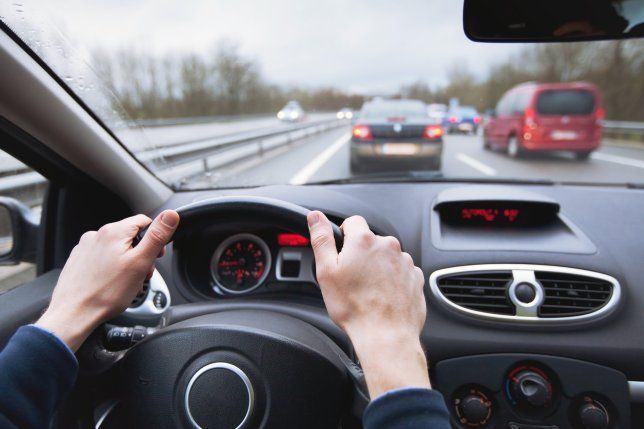
\includegraphics[height=0.35\linewidth]{Figuras/Ch15/fig1}
\end{frame}


\begin{frame}{Controle antecipativo (\textit{feedforward})}
	\begin{block}{}
		\begin{itemize}
			\item O controle \textbf{antecipativo} (também conhecido como \textit{antecipatório} ou \textit{preditivo}) é uma estratégia que se baseia na ideia de tentar \textbf{``prever'' os efeitos} de um distúrbio \textbf{antes} que este \textbf{afete o processo}.
			\item O controlador preditivo receberá o \textbf{sinal} do distúrbio e, usando alguma \textbf{ferramenta matemática}, vai gerar um sinal para \textbf{compensar a mudança} nas condições do processo.
			\item Geralmente é \textbf{associado ao controlador \textit{feedback}} por conta da sua \textbf{complementaridade}.
		\end{itemize}
	\end{block}

%	\vspace{0.5cm}

	\centering
	\scalebox{0.65}{
		\deftkzbds
		\begin{tikzpicture}[auto, node distance=1cm,>=Latex]
		\node[input] (in) {};
		\node[sum,right=2cm of in] (sum) {\Large $ + $};
		\node[block,right=of sum] (C) {Controlador FB};
		\node[sum,right=of C] (sum2) {\Large $ + $};
		\node[block, right=of sum2] (P) {Processo};
		\coordinate[right=of P] (mid);
		\node[output,right=of mid] (out) {};
		\node[block,below=of sum2] (S) {Sensor};
		\node[block,above=of C] (C2) {Controlador FF};
		\node[input,left=2cm of C2] (in2) {};
		
		\draw[->] (in) -- node[above,near start] {Entrada} (sum);
		\draw[->] (sum) -- (C);
		\draw[->] (C) -- (sum2);
		\draw[->] (in2) -- node[above,near start] {Distúrbio} (C2);
		\draw[->] (C2) -| (sum2);
		\draw[->] (sum2) -- (P);
		\draw[->] (mid) |- (S);
		\draw[->] (S) -| node[pos=0.98, xshift=15pt] {$-$} node[pos=1.21, xshift=-4pt] {$+$} (sum);
		\draw[->] (P) -- (out) node[above,near end] {Saída};
		\end{tikzpicture}}
\end{frame}


\begin{frame}{Controle antecipativo (\textit{feedforward})}
	\begin{block}{Controle antecipativo x ação derivativa}
		\begin{itemize}
			\item O controle antecipativo é \textbf{diferente} da ação derivativa.
			\item Enquanto a ação derivativa age \textbf{após} o aparecimento do erro, auxiliando na \textbf{resposta transitória} do controlador \textit{feedback}, o controlador \textit{feedforward} deve tentar corrigir a saída \textbf{antes} mesmo de o distúrbio ter atuado sobre o processo.
		\end{itemize}
	\end{block}
\end{frame}


\begin{frame}{Controle antecipativo (\textit{feedforward})}
	\begin{block}{Limitações}
		\begin{enumerate}
			\item Os distúrbios que não forem \textbf{medidos} não podem ser \textbf{controlados} nessa estratégia.
			\item O processo deve ter um \textbf{modelo matemático}, no mínimo, aproximado.
			\item O \textbf{ruído na medição} e as \textbf{imperfeições do modelo} matemático \textbf{não podem} ser eliminados por este controlador.
		\end{enumerate}
	\end{block}
\end{frame}


\begin{frame}{Controle antecipativo (\textit{feedforward})}
	\begin{block}{Semelhanças com o \textit{feedback}}
		Apesar das \textbf{diferenças} acentuadas (correção a partir da entrada, sem \textit{feedback}), há algumas \textbf{semelhanças} a serem notadas:
		\begin{enumerate}
			\item Ambas as malhas são \textbf{fechadas}.
			\item Em ambas as malhas há os \textbf{componentes básicos}: dispositivo de medição, controlador e válvula atuadora.
			\item O controlador é \textbf{essencialmente o mesmo} para ambas as malhas.
			\item Ambos controladores possuem \textbf{\textit{setpoint}}.
		\end{enumerate}
	\end{block}
\end{frame}


\begin{frame}{Controle antecipativo (\textit{feedforward})}
	\begin{block}{Aplicações}
		Nem todo processo requer a aplicação do	controle antecipatório. Inclusive, há processos onde a implementação do controle antecipatório é \textbf{impossível} ou \textbf{impraticável}.
		
		\medskip
		
		Como a implantação de um controle antecipatório requer o uso de vários instrumentos \textbf{adicionais}, a sua aplicação deve se \textbf{justificar economicamente}.
		
		\begin{enumerate}
			\item As \textbf{variações} nos \textbf{distúrbios} e \textbf{cargas de entrada} do processo levam um \textbf{tempo considerável} para afetar a variável controlada na saída, tornando \textbf{pouco eficiente} o controle convencional a realimentação negativa.
			\item É possível medir as variáveis de entrada que afetam \textbf{significativamente} a variável controlada com equipamentos disponíveis comercialmente.
			\item As \textbf{equações matemáticas finais} são resolvidas por equipamentos de controle, encontráveis no mercado e a custos \textbf{razoáveis}.
		\end{enumerate}
	\end{block}
\end{frame}


\begin{frame}{Controle antecipativo (\textit{feedforward})}
	\begin{block}{Exemplo \#02}
		\begin{itemize}
			\item O objetivo deste processo é controlar a \textbf{temperatura} ($ T_s $).
		\end{itemize}
	\end{block}

	\centering
	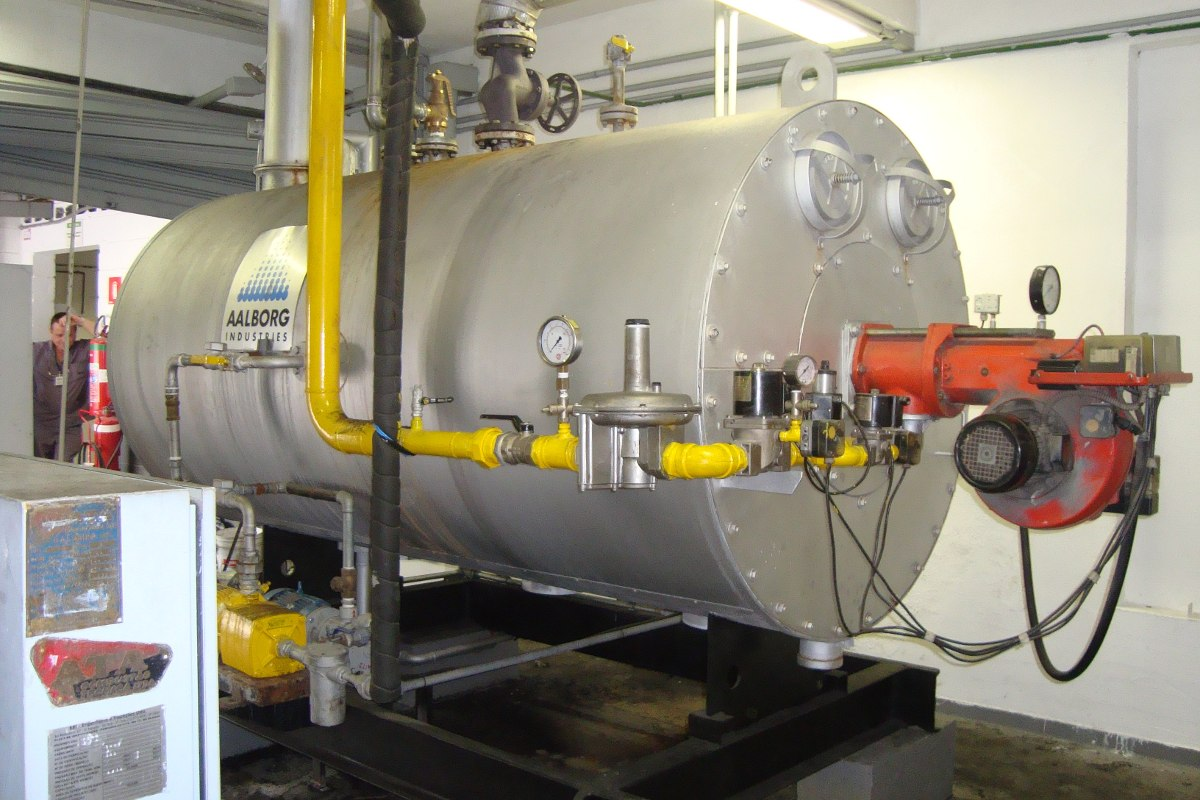
\includegraphics[width=0.7\linewidth]{Figuras/Ch15/fig3}

\end{frame}


\begin{frame}{Controle antecipativo (\textit{feedforward})}
	\begin{block}{Exemplo \#02}
		\begin{itemize}
			\item Para manter o \textbf{equilíbrio} do sistema, sabemos que para \textbf{diferentes valores} de vazão de entrada (carga) do fluido a ser aquecido, temos \textbf{diferentes posições de abertura} da válvula de controle (TCV).
			\item Admitindo-se que o sistema esteja \textbf{estável} no momento em que a carga \textbf{aumentar}, devemos \textbf{aumentar} também a \textbf{quantidade de combustível} que servirá para aquecer o forno.
		\end{itemize}
	\end{block}

	\centering
	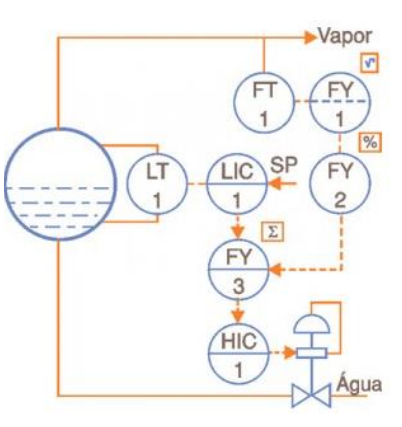
\includegraphics[height=0.5\textheight]{Figuras/Ch15/fig2}
\end{frame}


\begin{frame}{Controle antecipativo (\textit{feedforward})}
	\begin{block}{Exemplo \#02}
		\begin{itemize}
			\item Logo, se para realizar esta tarefa optarmos por uma malha de controle simples com apenas um controlador PID, assim que o \textbf{aumento de carga} ocorrer o controlador somente irá modificar a posição da válvula de controle (FCV) \textbf{depois} que \textbf{``sentir''} uma \textbf{diminuição no valor da temperatura} $ T_s $.
			\item Dependendo da \textbf{constante de tempo} do sistema (tempo de resposta), o processo tenderá a \textbf{oscilar}, tornando a temperatura $ T_s $ \textbf{instável}.
		\end{itemize}
	\end{block}
	
	\centering
	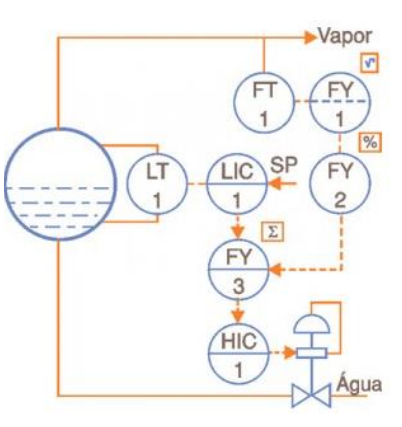
\includegraphics[height=0.45\textheight]{Figuras/Ch15/fig2}
\end{frame}


\begin{frame}{Controle antecipativo (\textit{feedforward})}
	\begin{block}{Exemplo \#02}
		\begin{itemize}
			\item No que se refere ao controle antecipativo, tão logo \textbf{aumente} a carga, um sinal \textbf{proporcional} a este aumento é enviado à malha de controle através do transmissor de vazão (FT1), onde é \textbf{somado} ao sinal de saída do controlador de temperatura (TIC) através do somador FY2, que por sua vez se encarregará de, antecipadamente, \textbf{adicionar mais combustível} ao sistema.
			\item Desta forma, a malha de controle antecipativo \textbf{``antecipa'' as variações medidas} já na entrada da variável controlada, e \textbf{impede} ou \textbf{minimiza} as \textbf{oscilações} no valor de temperatura da variável controlada $ T_s $.
		\end{itemize}
	\end{block}
\end{frame}


\begin{frame}{Controle em cascata}
	\begin{block}{Introdução}
		\begin{itemize}
			\item O controle em cascata consiste em \textbf{pelo menos duas malhas}, onde há uma \textbf{hierarquia} entre os \textbf{controladores}.
			\item Os controladores \textbf{mais acima} na hierarquia controlam os \textbf{pontos de ajuste} dos que estão diretamente abaixo, onde o \textbf{último} controla o processo \textbf{diretamente}.
			\item Essa estratégia \textbf{melhora a velocidade de resposta} da malha do processo e \textbf{reduz o impacto de distúrbios}.
			\item A malha de controle em cascata mais simples consiste em \textbf{dois controladores} com \textbf{realimentação negativa}, com a \textbf{saída} do controlador \textbf{primário} (mestre) estabelecendo o \textbf{ponto de ajuste} variável do \textbf{controle secundário} (escravo).
			\item Só é útil utilizar controladores em cascata quando houver uma \textbf{variável intermediária disponível} e que tenha \textbf{resposta mais rápida}.
		\end{itemize}
	\end{block}
\end{frame}


\begin{frame}{Controle em cascata}
	\begin{block}{Características}
		\begin{itemize}
			\item Quando os \textbf{períodos} das malhas primária e secundária são aproximadamente \textbf{iguais}, o sistema de controle fica \textbf{instável}, por causa das \textbf{variações simultâneas} do \textbf{ponto de ajuste} e da \textbf{medição} da malha secundária.
			\item Usualmente, o controlador \textbf{primário} é \textbf{PID} ou \textbf{PI} e o \textbf{secundário} é \textbf{PI}.
%			\item As combinações típicas das variáveis \textbf{primária (P)} e \textbf{secundária (S)} no controle em cascata são: temperatura (P) e vazão (S), composição (P) e vazão (S), nível (P) e vazão (S), temperatura (P) e pressão (S) e temperatura lenta (P) e temperatura rápida (S).
		\end{itemize}
	\end{block}

\medskip

\centering
\scalebox{0.6}{
	\deftkzbds
	\begin{tikzpicture}[auto, node distance=0.5cm,>=Latex]
	\node[input] (in) {};
	\node[sum,right=1.5cm of in] (sum) {\Large $ + $};
	\node[block,right=of sum] (C) {Controlador 1};
	\node[sum,right=0.5cm of C] (sum2) {\Large $ + $};
	\node[block,right=of sum2] (C2) {Controlador 2};
	\coordinate[right=of C2] (mid3);
	\node[block, right=of mid3] (P2) {Processo 2};
	\coordinate[right=of P2] (mid2);
	\node[block, right=of mid2] (P) {Processo 1};
	\coordinate[right=of P] (mid);
	\node[output,right=1.5cm of mid] (out) {};
	\coordinate[below=1.5cm of mid3] (il);
	\coordinate[below=2.5cm of mid3] (ol);
	
	\draw[->] (in) -- node[above,near start] {Entrada} (sum);
	\draw[->] (sum) -- (C);
	\draw[->] (C) -- (sum2);
	\draw[->] (sum2) -- (C2);
	\draw[->] (C2) -- (P2);
	\draw[->] (P2) -- (P);
	\draw[->] (mid) |- node[above left, midway] {malha externa} (ol);
	\draw[->] (ol) -| node[pos=0.98, xshift=15pt] {$-$} node[pos=1.17, xshift=-4pt] {$+$} (sum);
	\draw[->] (mid2) |- node[above left, midway] {malha interna} (il);
	\draw[->] (il) -| node[pos=0.98, xshift=15pt] {$-$} node[pos=1.26, xshift=-4pt] {$+$} (sum2);
	\draw[->] (P) -- (out) node[above,near end] {Saída};
	
	\draw[dashed] ($ (P2.south west)+(-10pt,-15pt) $) rectangle ($ (P.north east)+(10pt,10pt) $);
	\coordinate (n) at ($ (P.south)+(20pt,-17pt) $);
	\node[above] at (n) {Planta};
	\end{tikzpicture}}
\end{frame}


\begin{frame}{Controle em cascata}
	\begin{block}{Objetivos}
		\begin{enumerate}
			\item \textbf{Eliminar os efeitos} de alguns \textbf{distúrbios} (variações da carga próximas da fonte de suprimento).
			\item Melhorar o \textbf{desempenho dinâmico} (transitório) da malha de controle, reduzindo os efeitos do \textbf{atraso}, principalmente do \textbf{tempo morto}.
		\end{enumerate}
	\end{block}
\end{frame}


\begin{frame}{Controle em cascata}
	\begin{block}{Vantagens}
		\begin{itemize}
			\item Os distúrbios que afetam a \textbf{variável secundária} são \textbf{corrigidos} pelo \textbf{controlador secundário}, que é \textbf{mais rápido}, antes que possam influenciar a medição primária.
			\item O \textbf{atraso de fase} existente na parte \textbf{primária} é \textbf{reduzido} pela \textbf{malha secundária}, melhorando a velocidade de resposta da malha primária.
			\item A malha secundária permite uma \textbf{manipulação exata} da vazão de produto ou energia pelo \textbf{controlador primário}.
		\end{itemize}
	\end{block}
\end{frame}


\begin{frame}{Controle em cascata}
	\begin{block}{Exemplo \#01}
		\begin{itemize}
			\item Malha de controle em cascata com \textbf{malha escrava} controlando a \textbf{vazão} e \textbf{malha mestre} regulando a \textbf{temperatura de saída}.
		\end{itemize}
	\end{block}

	\centering
	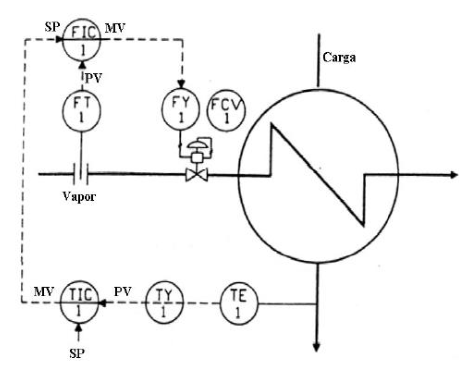
\includegraphics[width=0.6\linewidth]{Figuras/Ch15/fig4}
\end{frame}


\begin{frame}{Controle em cascata}
	\begin{block}{Exemplo \#02}
		\begin{itemize}
			\item Malha de controle em cascata com a malha \textbf{escrava} regulando a \textbf{temperatura de saída do fluido de aquecimento} e malha \textbf{mestre} regulando a \textbf{temperatura de reação química}.
		\end{itemize}
	\end{block}
	
	\centering
	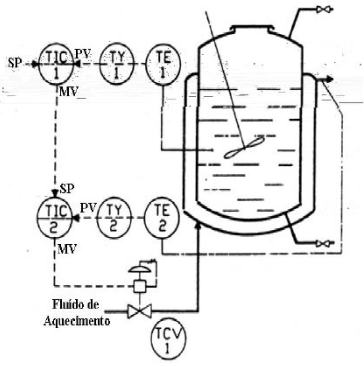
\includegraphics[width=0.45\linewidth]{Figuras/Ch15/fig5}
\end{frame}


\begin{frame}{Controle de relação}
	\begin{block}{Introdução}
		\begin{itemize}
			\item No controle de \textit{relação} (também chamado de \textit{razão}, \textit{fração} ou \textit{proporção}) o valor do \textit{setpoint} de uma das variáveis depende \textbf{diretamente} do valor de uma \textbf{segunda variável} de processo, normalmente denominada \textbf{variável piloto}.
			\item Basicamente, este controle serve para manter uma determinada \textbf{proporção} entre \textbf{dois ou mais} produtos.
		\end{itemize}
	\end{block}
\end{frame}


\begin{frame}{Controle de relação}
	\begin{block}{Exemplo \#01}
		\begin{itemize}
			\item A figura abaixo exemplifica isso trazendo uma aplicação onde se deseja obter um \textbf{refresco de fruta} a partir da vazão de \textbf{concentrado de suco} ($ Q_L $), e de uma determinada vazão de \textbf{água} ($ Q_A $).
		\end{itemize}
	\end{block}

	\vspace{0.3cm}

	\centering
	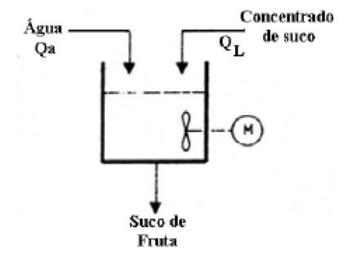
\includegraphics[width=0.5\linewidth]{Figuras/Ch15/fig10}
\end{frame}


\begin{frame}{Controle de relação}
	\begin{block}{Exemplo \#01}
		\begin{itemize}
			\item A relação $ k $ depende da \textbf{fórmula de fabricação}, a qual determina o sabor característico (que obviamente deve ser sempre o mesmo) do produto final do processo.
			\item Fica, portanto, evidente que \textbf{independentemente da variação} da vazão do concentrado de suco, o sistema deve ser capaz de \textbf{ajustar} o valor da vazão da água, \textbf{mantendo}, assim, a \textbf{relação} entre a água e o concentrado de suco.
		\end{itemize}
		
		\begin{align*}
		Q_A&=k\cdot Q_L\\
		k&=\dfrac{Q_A}{Q_L}
		\end{align*}
	\end{block}
\end{frame}


\begin{frame}{Controle de relação}
	\centering
	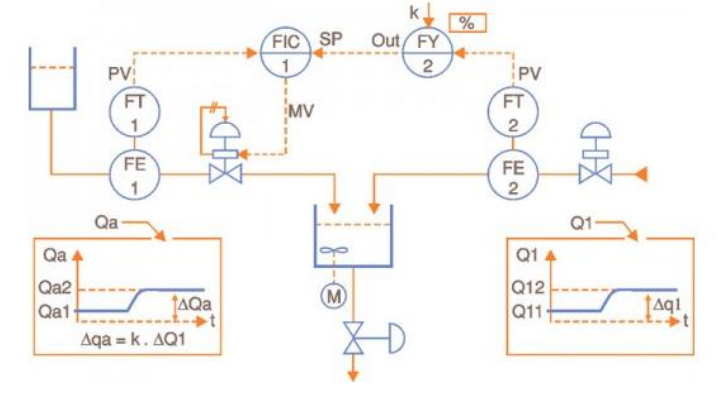
\includegraphics[width=0.9\linewidth]{Figuras/Ch15/fig6}
	
	\bigskip
	
	Malha completa
\end{frame}


\begin{frame}{Controle de relação}
	\begin{block}{Exemplo \#01}
		\begin{itemize}
			\item Através de um \textbf{elemento de medição de vazão} (FE2), o sistema mede o valor da \textbf{variável piloto}, neste caso o \textbf{concentrado de suco}, e envia o sinal para \textbf{FY}.
			\item Neste, temos a \textbf{multiplicação} do \textbf{fator de proporcionalidade da mistura} ($ k $) pelo valor de \textbf{vazão de concentrado de suco}.
			\item A saída deste bloco segue, então, diretamente para o \textbf{controlador de vazão de água} (FIC) que, por sua vez, tem como \textbf{\textit{setpoint}} o sinal \textbf{vindo de FY}.
			\item Desta forma, se o concentrado de suco sofrer alguma \textbf{alteração no valor de vazão}, teremos também uma \textbf{alteração} (de forma proporcional) no valor do \textbf{\textit{setpoint}} do \textbf{controlador de vazão de água} (FIC), que corrigirá \textbf{rapidamente} a quantidade de água que está sendo acrescentada na mistura, e como resultado final, a razão ($ k $) de água/concentrado de suco permanecerá \textbf{constante}.
		\end{itemize}
	\end{block}
\end{frame}


\begin{frame}{Controle de relação}
	\begin{block}{Aplicações}
		\begin{enumerate}
			\item Manter uma relação de \textbf{refluxo constante} em um \textbf{coluna de destilação}.
			\item Manter \textbf{quantidades estequiométricas} de dois reagentes sendo \textbf{alimentados} em um \textbf{reator}.
			\item \textbf{Misturar dois produtos}, como gasolina e álcool, numa \textbf{relação constante}.
		\end{enumerate}
	\end{block}
\end{frame}


\begin{frame}{Controle de relação}
	\begin{block}{Critérios para duas variáveis}
		O sistema é considerado de controle de relação quando:
		\begin{enumerate}
			\item As \textbf{duas} variáveis \textbf{X} e \textbf{Y} são \textbf{medidas}.
			\item \textbf{Apenas uma} das duas variáveis é manipulada, por exemplo X.
			\item A variável realmente \textbf{controlada} é a \textbf{relação} $ \bm{k} $ entre as duas variáveis X e Y.
		\end{enumerate}
	\end{block}
\end{frame}


%\begin{frame}{Controle de relação}
%	\centering
%	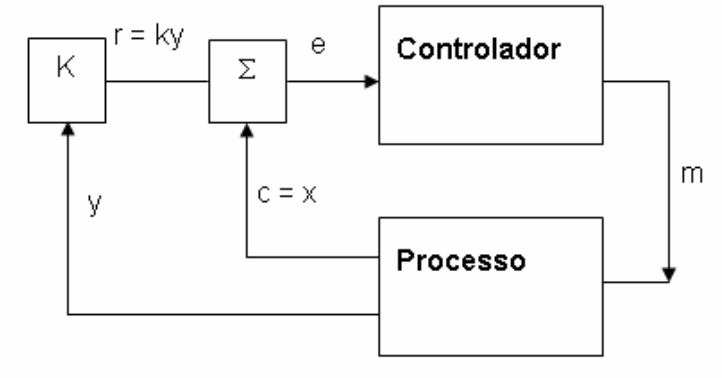
\includegraphics[width=0.7\linewidth]{Figuras/Ch15/fig7}
%	
%	\medskip
%	
%	Diagrama de blocos do controle de relação
%	
%	\begin{block}{Observação}
%		\begin{itemize}
%			\item A álgebra é feita \textbf{fora do controlador} para evitar \textbf{problemas de ganho} e, como consequência, de \textbf{estabilidade}.
%		\end{itemize}
%	\end{block}
%\end{frame}


\begin{frame}{Controle de relação}
	\begin{block}{Critérios para $ n $ variáveis}
		\begin{itemize}
			\item Quando se tem o controle de relação de \textbf{várias} ($ n $) \textbf{vazões}, uma delas deve ser \textbf{livre} e as \textbf{outras} ($ n-1 $) são \textbf{manipuladas}. Sempre devendo haver \textbf{pelo menos um grau de liberdade}.
			\item Os valores monitorados são o \textbf{ponto de ajuste} (relação) e os valores medidos das $ \bm{n} $ \textbf{vazões}.
			\item A soma das relações é sempre igual a $ \bm{100\%} $ ou, na forma normalizada, igual a $ \bm{1} $.
		\end{itemize}
	\end{block}
\end{frame}


\begin{frame}{Controle de relação}
	\begin{block}{Exemplo \#02}
		\begin{itemize}
			\item O controlador do misturador de massa com água recebe informações de FT1 e FT2, através dos quais realiza o controle da vazão de água ($ Q_a $) através do controle da válvula.
		\end{itemize}
	\end{block}

	\centering
	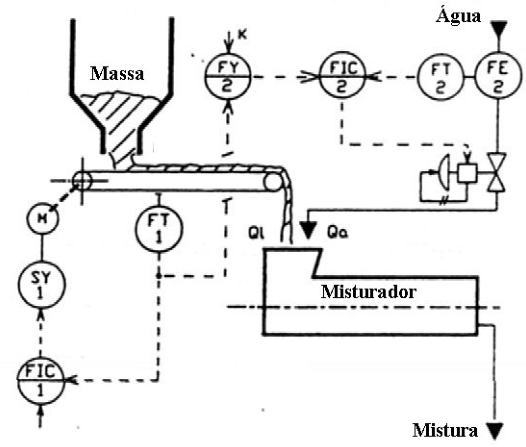
\includegraphics[width=0.5\linewidth]{Figuras/Ch15/fig8}
\end{frame}


\begin{frame}{Controle de relação}
	\begin{block}{Junção dos controles de relação e de cascata}
		\begin{itemize}
			\item A e B são as duas vazões que \textbf{alimentam} o tanque.
			\item O nível do liquido é afetado pela \textbf{vazão total}, por isso o controlador de nível (LC) \textbf{cascateia o controlador da vazão A} (FC1), ou seja, o \textbf{ponto de ajuste} do controlador da vazão A é estabelecido pela \textbf{saída do controlador de nível do tanque}.
		\end{itemize}
	\end{block}
	
	\centering
	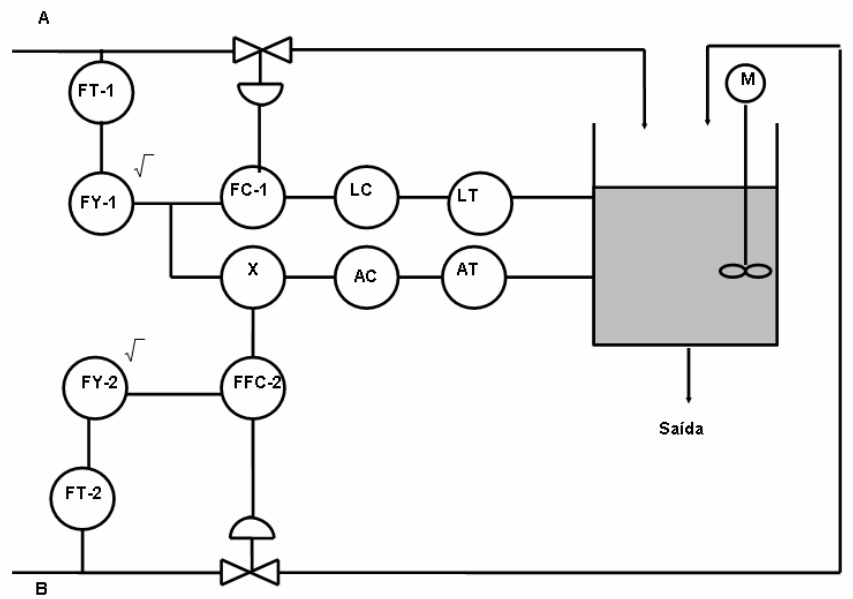
\includegraphics[width=0.5\linewidth]{Figuras/Ch15/fig9}
\end{frame}


\begin{frame}{Controle de relação}
	\begin{block}{Junção dos controles de relação e de cascata}
		\begin{itemize}
			\item A vazão A, por sua vez, se relacionada com a vazão B, já que \textbf{ambos os produtos} devem manter uma \textbf{relação} na mistura.
			\item Esse controle é feito pelo \textbf{controlador de relação de vazão} (FFC2), que atua na \textbf{vazão B}.
		\end{itemize}
	\end{block}
	
	\centering
	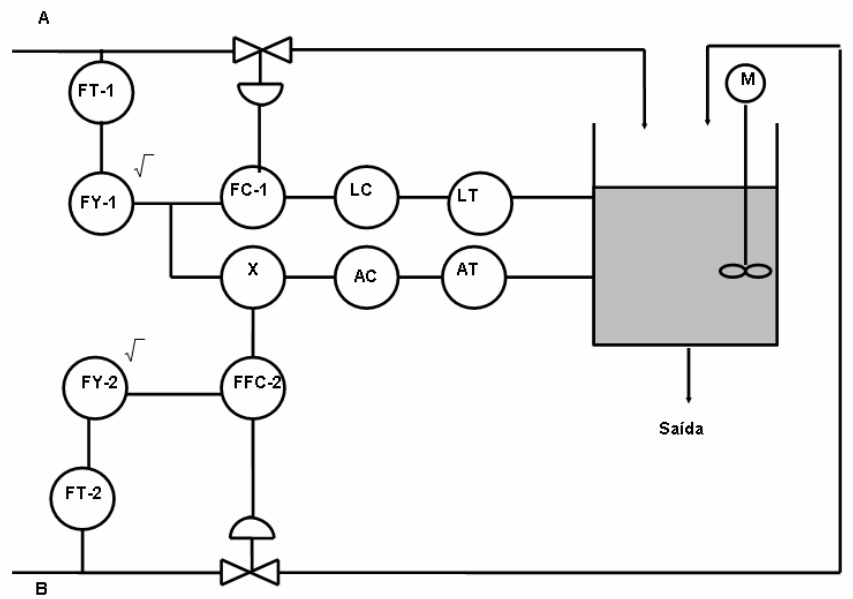
\includegraphics[width=0.55\linewidth]{Figuras/Ch15/fig9}
\end{frame}


\begin{frame}{Controle de relação}
	\begin{block}{Junção dos controles de relação e de cascata}
		\begin{itemize}
			\item Para \textbf{diminuir o efeito} desse controlador no nível do líquido, a vazão B deve ser \textbf{a menor das duas vazões}, já que \textbf{não deve} influenciar no \textbf{nível do tanque}, e sim na \textbf{composição da mistura}, a fim de não causar \textbf{instabilidade} na malha externa.
		\end{itemize}
	\end{block}
	
	\centering
	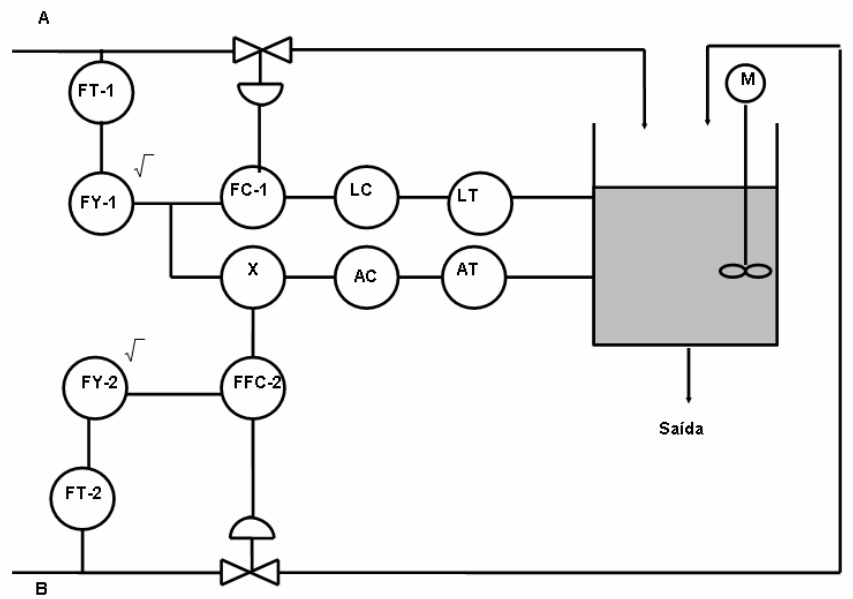
\includegraphics[width=0.55\linewidth]{Figuras/Ch15/fig9}
\end{frame}


%\begin{frame}{Controle de relação}
%	\centering
%	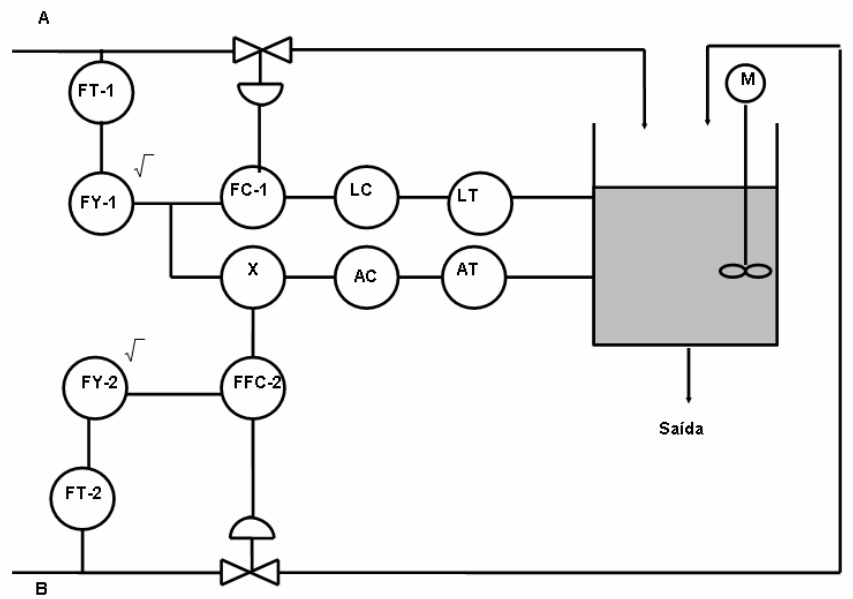
\includegraphics[width=0.7\linewidth]{Figuras/Ch15/fig9}
%	
%	\bigskip
%	
%	Malha combinando controles de relação e de cascata
%\end{frame}


\begin{frame}{Controle de faixa dividida (\textit{split-range})}
	\begin{block}{Introdução}
		\begin{itemize}
			\item O controle de faixa dividida (\textit{split-range}) consiste em \textbf{um único controlador} manipulando \textbf{dois ou mais elementos finais de controle}.
			\item Neste controle é mandatório o uso do \textbf{posicionador da válvula}, que é um acessório que \textbf{garante o posicionamento correto} da \textbf{haste da válvula}, dando-a também \textbf{outras funcionalidades}.
		\end{itemize}
	\end{block}

	\centering
	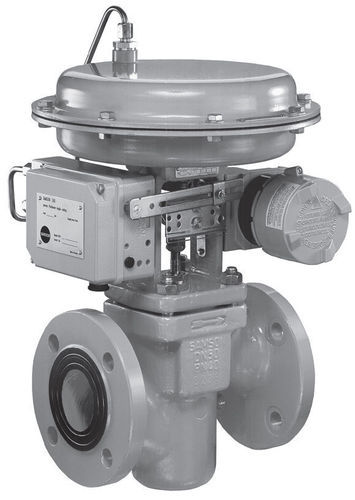
\includegraphics[height=0.45\textheight]{Figuras/Ch15/fig15}
\end{frame}


\begin{frame}{Controle de faixa dividida (\textit{split-range})}
	\begin{block}{Introdução}
		\begin{itemize}
			\item Os posicionadores são \textbf{calibrados} e \textbf{ajustados} e as \textbf{ações das válvulas} são escolhidas para que os elementos finais de controle sejam \textbf{manipulados convenientemente}.
			\item Por exemplo, uma válvula pode operar de \textbf{0 a 50\%} do sinal e a outra de \textbf{50 a 100\%} do sinal de saída do controlador.
			\item Esta montagem é utilizada:
			\begin{enumerate}
				\item\normalsize Quando a \textbf{rangeabilidade necessária} para uma aplicação é \textbf{maior} que a \textbf{rangeabilidade de um único elemento final de controle}.
				\item\normalsize Quando é necessário utilizar \textbf{dois} elementos finais de controle \textbf{indiferentemente da situação}.
			\end{enumerate}
		\end{itemize}
	\end{block}
\end{frame}


\begin{frame}{Controle de faixa dividida (\textit{split-range})}
	\begin{block}{Aplicações - exemplo \#01 - aquecimento e resfriamento}
		\begin{itemize}
			\item A figura abaixo mostra um esquema de \textbf{controle de temperatura} para um processo em \textbf{bateladas} (\textit{batches}), usando um tanque de reação química que requer a \textbf{temperatura de reação constante}.
		\end{itemize}
	\end{block}
	
	\centering
	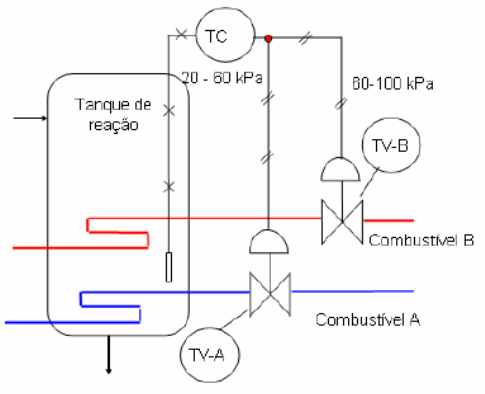
\includegraphics[width=0.55\linewidth]{Figuras/Ch15/fig11}
\end{frame}


\begin{frame}{Controle de faixa dividida (\textit{split-range})}
	\begin{block}{Aplicações - exemplo \#01 - aquecimento e resfriamento}
		Para começar, a reação o tanque deve ser \textbf{aquecido} e isto requer uma \textbf{vazão de vapor} através da serpentina.
		
		\medskip
		
		Depois, a reação exotérmica produz \textbf{calor} e o tanque deve ser \textbf{resfriado} e isto requer uma \textbf{vazão de fluido refrigerante}, através de outra (ou da mesma) serpentina.
		
		\medskip
		
		O controle suave da temperatura é alcançado pelo seguinte sistema básico:
		\begin{itemize}
			\item A saída do controlador de temperatura varia \textbf{gradualmente} quando a temperatura do tanque \textbf{aumenta}.
		\end{itemize}
	\end{block}
\end{frame}


\begin{frame}{Controle de faixa dividida (\textit{split-range})}
	\begin{block}{Aplicações - exemplo \#01 - aquecimento e resfriamento}
		\begin{itemize}
			\item Quando o controlador solicita que a \textbf{válvula de aquecimento} esteja \textbf{totalmente aberta}, a \textbf{válvula de resfriamento} deve estar \textbf{totalmente fechada}.
			\item Quando o controlador solicita que a \textbf{válvula de resfriamento} esteja \textbf{totalmente aberta}, a \textbf{válvula de aquecimento} deve estar \textbf{totalmente fechada}.
		\end{itemize}
	\end{block}

	\centering
	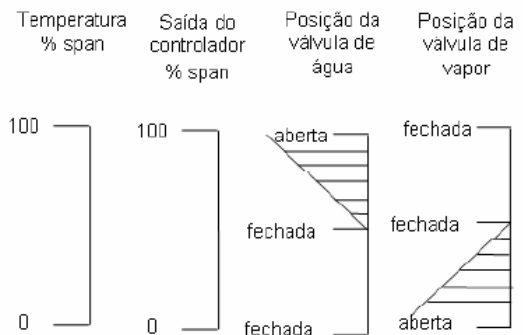
\includegraphics[width=0.5\linewidth]{Figuras/Ch15/fig12}
\end{frame}


\begin{frame}{Controle de faixa dividida (\textit{split-range})}
	\begin{block}{Aplicações - exemplo \#01 - aquecimento e resfriamento}
		\begin{itemize}
			\item \textbf{No meio do caminho}, \textbf{ambas as válvulas} devem estar \textbf{simultaneamente fechadas}, de modo que não haja \textbf{nem aquecimento nem resfriamento}.
			\item Cada válvula se move de \textbf{modo contrário e sequencial} à outra.
		\end{itemize}
	\end{block}
	
	\centering
	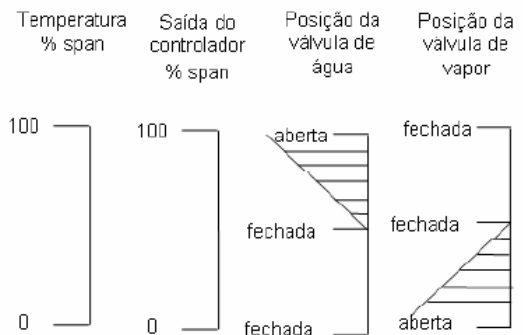
\includegraphics[width=0.6\linewidth]{Figuras/Ch15/fig12}
\end{frame}


\begin{frame}{Controle de faixa dividida (\textit{split-range})}
	\begin{block}{Aplicações - exemplo \#02 - temperatura com dois combustíveis}
		\begin{itemize}
			\item Também há aplicações envolvendo o aquecimento por \textbf{dois combustíveis}, onde a primeira válvula A (do combustível \textbf{mais barato}) é atuada pela saída do controlador, indo de \textbf{0 a 100\%} de abertura.
			\item Depois de \textbf{totalmente aberta}, a segunda válvula B (do combustível \textbf{mais caro}) \textbf{começa a atuar}, indo também de \textbf{0 a 100\%}.
		\end{itemize}
	\end{block}

	\centering
	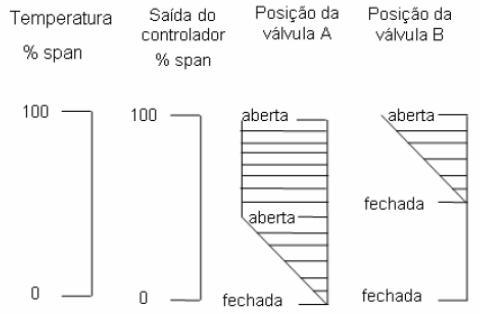
\includegraphics[width=0.5\linewidth]{Figuras/Ch15/fig13}
\end{frame}


\begin{frame}{Controle de faixa dividida (\textit{split-range})}
	\begin{block}{Aplicações - exemplo \#02 - temperatura com dois combustíveis}
		\begin{itemize}
			\item Neste caso, pode-se ter as duas válvulas \textbf{totalmente fechadas} (no início do processo) ou \textbf{totalmente abertas}, (no máximo aquecimento) \textbf{simultaneamente}.
		\end{itemize}
	\end{block}
	
	\centering
	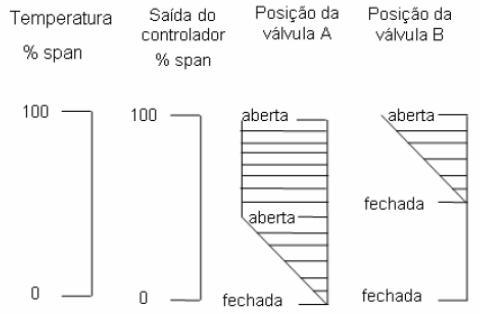
\includegraphics[width=0.7\linewidth]{Figuras/Ch15/fig13}
\end{frame}


%\begin{frame}{Controle de faixa dividida (\textit{split-range})}
%	\centering
%	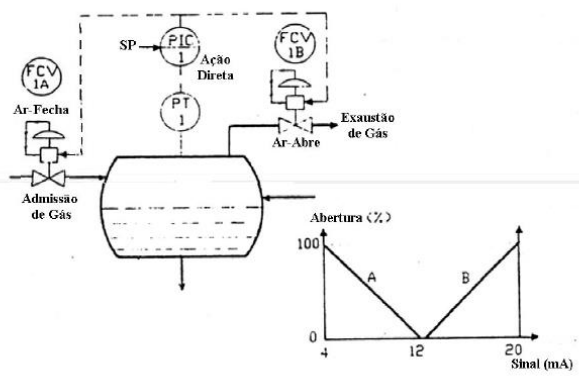
\includegraphics[width=0.7\linewidth]{Figuras/Ch15/fig14}
%	
%	\bigskip
%	
%	Controle de pressão
%\end{frame}


\frame{
	\frametitle{Exercícios}
	\begin{block}{}
		01. Como ocorrem as correções numa malha com um controlador antecipativo? Por que utilizá-lo?
		
		\vspace{0.5cm}
		
		02. Desenhe um diagrama PI de um processo com estratégia de controle em cascata.
		
		\vspace{0.5cm}
		
		03. Dado um forno com \SI{300}{\liter} de capacidade, sabendo que dispõe de válvulas com \SI{1.5}{\liter\per\minute} de vazão e o forno queima \SI{3}{\liter\per\minute} em capacidade máxima, qual estratégia de controle é mais apropriada? Desenhe um diagrama para este processo.
	\end{block}
}


\section*{Referências}
\frame{
	\frametitle{Referências e Exercícios Complementares}
	\begin{itemize}
		\item BAYER, Fernando Mariano; ARAÚJO, Olinto César Bassi de. Controle Automático de Processos, 3 ed. UFSM : Colégio Técnico Industrial de Santa Maria, 2011.
	\end{itemize}
	%\centering{\alert{Página 546 - \textbf{Capítulo 6}}} \\
	%\centering{\alert{Lista de exercícios 01}}
}